\documentclass[10pt,twocolumn,letterpaper]{article}
\usepackage[review]{cvpr}
\usepackage{microtype}
\usepackage{booktabs}
\usepackage{amsmath,amssymb}
\definecolor{cvprblue}{rgb}{0.21,0.49,0.74}
\usepackage[pagebackref,breaklinks,colorlinks,allcolors=cvprblue]{hyperref}
\hypersetup{pdftitle={Restoring Native CT Evidence at Fixed Proposals for Lung Nodule Ranking},
            pdfauthor={},pdfsubject={Anonymous CVPR review}}
\newcommand{\mm}{\,\mathrm{mm}}
\newcommand{\HU}{\,\mathrm{HU}}
\newcommand{\pos}[1]{\left[#1\right]_+}
\newcommand{\EvalScans}{353}
\newcommand{\EvalMarks}{301,306}
\newcommand{\EvalLesions}{461}
\newcommand{\ProposedLesions}{455}
\newcommand{\BallCpm}{83.58}
\newcommand{\BandCpm}{87.60}
\newcommand{\FullCpm}{89.37}
\newcommand{\RestorePrimary}{$+4.03\,[1.85,\,6.17]$}
\newcommand{\RestorePrimaryPointwise}{$+4.03\,[2.16,\,5.71]$}
\newcommand{\RestoreRepeat}{$+4.21\,[2.51,\,6.17]$}
\newcommand{\RestoreOne}{$+4.12\,[1.45,\,6.71]$}
\newcommand{\RepeatOne}{$+3.47\,[0.67,\,6.59]$}
\newcommand{\PrimaryOneGain}{4.12}
\newcommand{\RepeatOneGain}{3.47}
\newcommand{\RestoreGain}{+4.03}
\newcommand{\RepeatGain}{+4.21}
\newcommand{\PrimaryRecovery}{70}
\newcommand{\RepeatRecovery}{73}
\newcommand{\TriGain}{$+1.27\,[-0.71,\,3.58]$}
\newcommand{\TriOne}{$+0.22\,[-2.49,\,2.88]$}
\newcommand{\SingleGain}{$+2.91\,[0.69,\,5.48]$}
\newcommand{\SingleEstimate}{2.91}
\newcommand{\SingleOne}{$+0.87\,[-2.59,\,4.73]$}
\newcommand{\SingleCheck}{84.59}
\newcommand{\SingleDev}{81.70}
\newcommand{\QuerySources}{2,849}
\newcommand{\BandSources}{16,672}
\newcommand{\SourcesGain}{$+1.74\,[-0.21,\,3.12]$}
\newcommand{\SourcesOne}{$+2.60\,[-0.63,\,4.64]$}
\newcommand{\CoverageGap}{$+2.29\,[0.94,\,4.13]$}
\newcommand{\CoverageOne}{$+1.52\,[-0.47,\,4.73]$}
\newcommand{\AnyOverlap}{72}
\newcommand{\NeverOverlap}{377}
\newcommand{\AnyPrimary}{$+15.28\,[5.81,\,25.00]$}
\newcommand{\AnyRepeat}{$+16.67\,[6.85,\,26.09]$}
\newcommand{\NeverPrimary}{$+2.12\,[-0.52,\,4.79]$}
\newcommand{\NeverRepeat}{$+1.06\,[-1.68,\,4.27]$}
\newcommand{\HeteroPrimary}{$+13.16\,[3.68,\,22.85]$}
\newcommand{\HeteroRepeat}{$+15.61\,[4.69,\,24.92]$}
\newcommand{\RepresentPrimary}{$+0.62\,[-0.09,\,1.38]$}
\newcommand{\RepresentRepeat}{$-0.19\,[-0.72,\,0.60]$}
\newcommand{\FusionPrimary}{$-0.09\,[-1.23,\,1.05]$}
\newcommand{\PairShamPrimary}{$-0.03\,[-0.68,\,0.51]$}
\newcommand{\PairShamRepeat}{$-0.11\,[-0.71,\,0.54]$}
\newcommand{\PairUnpairedPrimary}{$-0.31\,[-0.94,\,0.30]$}
\newcommand{\PairUnpairedRepeat}{$-0.31\,[-1.02,\,0.41]$}
\newcommand{\PracticalPrimary}{$+0.22\,[-0.29,\,0.50]$}
\newcommand{\PracticalRepeat}{$-0.19\,[-0.86,\,0.41]$}
\newcommand{\PracticalOne}{$+0.65\,[-0.67,\,1.14]$}
\newcommand{\PracticalRepeatOne}{$-0.22\,[-1.25,\,1.10]$}
\newcommand{\TransferredPrimary}{$+3.69\,[1.02,\,6.53]$}
\newcommand{\TransferredRepeat}{$+2.39\,[-0.22,\,5.03]$}
\newcommand{\PrimaryUncapped}{$+4.03\,[2.16,\,5.71]$}
\newcommand{\RepeatUncapped}{$+4.21\,[2.52,\,6.19]$}
\newcommand{\GeometrySmallPrimary}{$+0.19\,[-0.56,\,0.83]$}
\newcommand{\GeometryLargePrimary}{$-0.15\,[-0.63,\,0.22]$}
\newcommand{\CapacityBlindPrimary}{$+0.15\,[-0.49,\,0.82]$}
\newcommand{\CapacitySpatialPrimary}{$-0.19\,[-0.79,\,0.44]$}
\newcommand{\DirectionalSmallPrimary}{$+0.99\,[0.03,\,1.47]$}
\newcommand{\DirectionalLargePrimary}{$+0.81\,[0.09,\,1.11]$}
\newcommand{\RefitPrimary}{$+0.62\,[-0.15,\,1.02]$}
\newcommand{\CompactGapPrimary}{$+2.54\,[1.05,\,4.57]$}
\newcommand{\ResidualSmallPrimary}{$+3.04\,[1.44,\,5.04]$}
\newcommand{\ResidualLargePrimary}{$+3.22\,[1.58,\,5.12]$}
\newcommand{\GeometrySmallOnePrimary}{$-0.65\,[-2.52,\,1.04]$}
\newcommand{\GeometryLargeOnePrimary}{$-0.87\,[-1.78,\,0.00]$}
\newcommand{\ResidualSmallOnePrimary}{$+3.47\,[0.72,\,6.53]$}
\newcommand{\ResidualLargeOnePrimary}{$+3.25\,[0.83,\,5.90]$}
\newcommand{\GeometrySmallRepeat}{$-0.22\,[-0.46,\,0.25]$}
\newcommand{\GeometryLargeRepeat}{$+0.00\,[0.00,\,0.07]$}
\newcommand{\CapacityBlindRepeat}{$+0.00\,[-0.06,\,0.03]$}
\newcommand{\CapacitySpatialRepeat}{$+0.22\,[-0.24,\,0.46]$}
\newcommand{\DirectionalSmallRepeat}{$-0.22\,[-0.46,\,0.24]$}
\newcommand{\DirectionalLargeRepeat}{$+0.00\,[0.00,\,0.03]$}
\newcommand{\RefitRepeat}{$-0.03\,[-0.80,\,0.46]$}
\newcommand{\CompactGapRepeat}{$+4.12\,[2.33,\,5.95]$}
\newcommand{\ResidualSmallRepeat}{$+4.43\,[2.63,\,6.39]$}
\newcommand{\ResidualLargeRepeat}{$+4.21\,[2.51,\,6.17]$}
\newcommand{\GeometrySmallOneRepeat}{$+0.22\,[-0.64,\,1.10]$}
\newcommand{\GeometryLargeOneRepeat}{$+0.00\,[0.00,\,0.00]$}
\newcommand{\ResidualSmallOneRepeat}{$+3.25\,[0.42,\,6.42]$}
\newcommand{\ResidualLargeOneRepeat}{$+3.47\,[0.67,\,6.59]$}


\def\paperID{}
\def\confName{CVPR}
\def\confYear{2027}
\title{Restoring Native CT Evidence at Fixed Proposals for Lung Nodule Ranking}
\author{Anonymous CVPR submission}

\begin{document}
\maketitle
\begin{abstract}
We test what a candidate-centered band of native CT can add to lung nodule ranking. At each released proposal we preserve a $10\mm$ ball and restore a band around it before interpolation. On \EvalScans{} reused LUNA16 scans, the primary two-scale 3D ranker rises from \BallCpm\% to \BandCpm\% CPM, a gain of \RestorePrimary{} points with a multiplicity-adjusted patient interval. A second fit gains \RestoreRepeat{} points with a pointwise interval. Matched sensitivity at 1 false positive per scan rises by \PrimaryOneGain{} and \RepeatOneGain{} points. Two controls clarify the dense advantage. Relative angular attention on the same 384 exterior readings leaves a multi-point gap. Even when the exact native sources of those readings enter the same image encoder as the band, the band leads by \CoverageGap{} CPM points. The matched sensitivity gains are largest among lesions whose majority-reader contour can be reached by the band at a matching proposal. A distinct single-stream 3D model also gains \SingleEstimate{} CPM points. These results locate useful evidence in the added native coverage and show that a proposal-centered exterior can restore target tissue as well as surrounding anatomy.

\end{abstract}

\section{Introduction}

At a candidate location in a chest CT, a nodule and the cross-section of a vessel can both appear as a compact bright object. A larger field can reveal continuation along the vessel. It can also restore part of a nodule whose center is displaced from the candidate or whose boundary extends beyond the local view. A ranking gain from a larger field leaves both explanations open. To learn what the additional field makes available, we need to control access to the original scan while holding the proposals and the ranking task fixed.

We preserve the native voxels in a $10\mm$ ball around every proposal and restore a nearby band while keeping the input grid, network and training recipe fixed. The band contains the native source voxels of a set of sparsely sampled exterior intensity readings. Masking the original voxels before trilinear resampling gives the ball and band conditions the same interior sources and makes the intended access difference explicit. Each fit learns under the visibility it will receive at evaluation. This tests whether the newly accessible evidence can improve ranking under matched training.

On the \EvalScans{} reused LUNA16 scans, the band raises the primary two-scale 3D ranker from \BallCpm\% to \BandCpm\% competition performance metric (CPM). The paired increase is \RestorePrimary{} points with the original multiplicity adjustment. A second fit gains \RestoreRepeat{} points with a pointwise interval. At a matched 1 false positive (FP) per scan, sensitivity improves by \PrimaryOneGain{} and \RepeatOneGain{} points. The band recovers \PrimaryRecovery\% and \RepeatRecovery\% of their observed full-minus-ball CPM gaps. This places a substantial fraction of the fitted models' context advantage within a physically specified set of native sources.

We use three complementary comparisons to explain the gain. First, we give matched sparse readouts the same 384 intensity readings with or without information about neighboring directions, and vary their capacity while holding the image score and fusion point fixed. Second, we expose the exact native sources of the sparse queries to the two-scale image encoder itself, where they enter at the same layer as the full band. This tests whether a gap survives when the sparse source locations participate in the same end-to-end image computation. Third, we use existing reader contours to locate which lesions could be touched by the band at any of their matching proposals. The subgroup analysis separates access to annotated lesion tissue from access beyond that tissue at those proposals.

These comparisons turn a single dense-versus-pooled result into a set of tests of access, representation and anatomy. We also repeat ball, band and full fitting in a distinct single-stream 3D architecture to test how the effect transfers under the same proposal stream. The resulting evidence concerns fixed-proposal ranking on a previously examined benchmark, where the candidate generator and the reference denominator are shared across all visibility conditions.

\begin{figure*}[t]
  \centering
  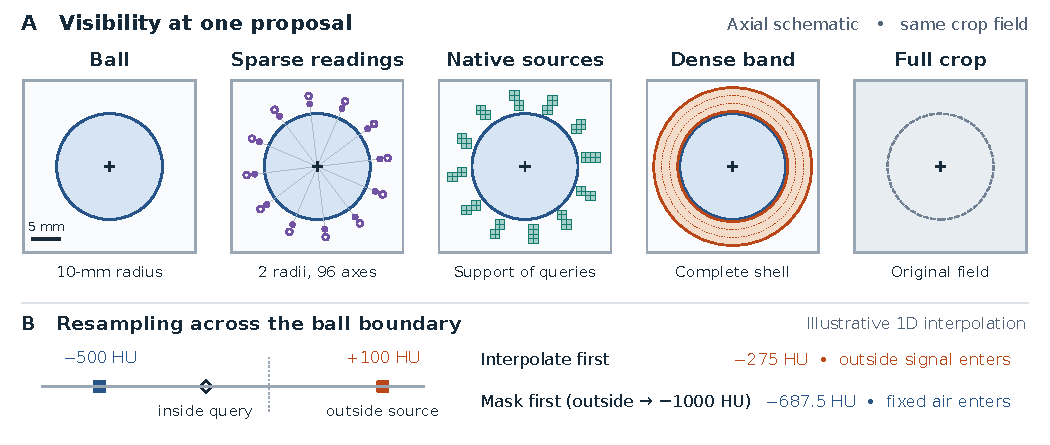
\includegraphics[width=\textwidth]{figures/visibility.pdf}
  \caption{Five ways to expose evidence at the same physical proposal (cross). Blue preserves the native ball. The sparse head receives two samples on each arm of each of 96 axes in 3D, shown here by a subset of in-plane queries. The native-source condition gives the image encoder the voxel values supporting those interpolated queries. The dense band retains the entire bounded radial support, and the full condition uses the original field. Hidden native intensities become fixed air before sampling the same centered crop. A uses an illustrative native spacing. B shows how interpolating first would carry signal from an exterior voxel into an interior query. Masking first replaces that signal with a fixed contribution from air.}
  \label{fig:visibility}
\end{figure*}

\section{Related work}

\paragraph{Shape and exterior measurements.}
Hessian enhancement separates dot-like nodules from lines and sheets at candidate sites~\cite{li2003selective}. Van de Leemput \etal apply a spherical-shell feature after candidate generation to separate vascular and nodular structures~\cite{leemput2015shell}. Ciompi \etal sample circular intensity profiles on multiscale spherical surfaces and describe nodules by pooling their frequency spectra~\cite{ciompi2015frequencies}. These studies establish the relevance of exterior measurements and structured shape cues. We use the query locations to define an access intervention, compare a subset of native sources with its encompassing band, and measure how much ranking improves before selecting an exterior descriptor.

\paragraph{Learned context at fixed candidates.}
Setio \etal combine evidence from differently oriented planes with multistream CNNs for false-positive reduction~\cite{setio2016multiview}. Kim \etal use nested fields of view and learn gradual integration of features across scales~\cite{kim2018mgi}. The LUNA16 false-positive reduction track makes comparisons at common candidates possible~\cite{setio2017luna16}. Under that setup, our dense visibility comparisons vary the original CT sources available to a model, including the sources that contribute to the inner resampled grid. We keep the field of view and its tensor shape constant. This makes the band intervention distinct from choosing a wider patch or introducing another stream.

\paragraph{Geometry and set readouts.}
Permutation-invariant pooling summarizes a set of measurements without arbitrary row order~\cite{zaheer2017deep}. Set attention extends such readouts with learned interactions across elements~\cite{lee2019set}. We use the same set computation with and without a relative angular bias. This leaves the opposing pair identity within each row intact and isolates whether cross-row directional structure helps under a common sparse fusion scheme.

\section{Controlling what the ranker can see}
\label{sec:visibility}

\subsection{Setting and notation}
\label{sec:setting}

A scan is a set of native voxel centres $v\in\mathbb{R}^3$ (in millimetres, physical coordinates) with intensities $I(v)$ in Hounsfield units (HU). The candidate generator supplies proposals $p\in\mathbb{R}^3$; we use the released LUNA16 proposals unchanged~\cite{setio2017luna16}. For each proposal, a ranker receives a crop and returns a score. The crop is a $32^3$ grid centred at $p$ and aligned with the native axes, with $1.2\mm$ spacing, obtained by trilinear interpolation of the native voxels. Values are clipped to $[-1000,400]\HU$ and stored as 8-bit integers; the networks use the central $28^3$ samples, which span $32.4\mm$. All conditions below share this crop, so the input shape never changes.

\subsection{Mask native voxels, then resample}
\label{sec:mask}

A \emph{visibility condition} is a set $V$ of native voxels the ranker may see. All other voxels are replaced by air:
\begin{equation}
 I_V(v)=
 \begin{cases}
 I(v), & v\in V,\\
 -1000\HU, & v\notin V .
 \end{cases}
 \label{eq:mask}
\end{equation}
The crop is then resampled from $I_V$. The order matters. Trilinear interpolation mixes up to eight neighbouring native voxels, so masking the \emph{resampled} grid would let a hidden voxel near the boundary leak into a visible sample. With Eq.~\eqref{eq:mask}, a hidden voxel contributes only the constant value of air (Fig.~\ref{fig:visibility}b). \paragraph{Implementation checks.} For speed, masking is applied to a cropped neighbourhood of each proposal rather than to the whole scan, with a margin of native voxels kept for interpolation. We compared this implementation with literal whole-volume masking in nine test settings that include rotated, reflected and anisotropic native grids and proposals near the scan boundary. The crops were bit-identical. Replacing all 485,801 hidden voxel values in these settings with random values also left every crop and every sparse sample unchanged, and all 15,664 positive-weight interpolation contributions fell inside the visible set. The network receives no separate visibility channel; hidden regions appear only as air (supplement Sec.~S2).

The three main conditions use the ball
\begin{equation}
B(p)=\{v:\lVert v-p\rVert\le 10\mm\},
\end{equation}
the ball plus a band $A(p)$ defined next, and the full field.

\subsection{The band: where sparse samples get their values}
\label{sec:band}

Let $d$ be the diagonal of one native voxel, which depends on the scan's spacing. Any native voxel with a positive trilinear weight for a sample point $q$ lies within $d$ of $q$. We place sparse samples at two radii from the proposal,
\begin{equation}
 \begin{aligned}
 r_N &=10\mm+\max(1.9\mm,\,d+0.05\mm),\\
 r_F &=r_N+1.5\mm .
 \end{aligned}
 \label{eq:radii}
\end{equation}
By the triangle inequality, every native voxel $v$ that contributes to a sample at either radius satisfies
\begin{equation}
 r_N-d\;\leq\;\lVert v-p\rVert\;\leq\;r_F+d .
 \label{eq:support}
\end{equation}
The band is exactly this shell of native voxels,
\begin{equation}
A(p)=\{v:\ r_N-d\le\lVert v-p\rVert\le r_F+d\}.
\label{eq:band}
\end{equation}
Because $r_N-d\ge10.05\mm$, the band never overlaps the ball, and a thin gap of air separates them. For example, with $0.70\times0.70\times1.25\mm$ voxels, $d=1.59\mm$, $r_N=11.9\mm$, $r_F=13.4\mm$, and the band covers $10.3$--$15.0\mm$. The construction adapts to each scan's spacing, so Eq.~\eqref{eq:support} holds for every slice thickness. Algorithm~\ref{alg:band} summarizes the procedure.

\begin{algorithm}[t]
\caption{Building one visibility-controlled input}
\label{alg:band}
\small
\begin{algorithmic}[1]
\Require scan $\{(v,I(v))\}$, voxel spacing $s$, proposal $p$, condition $c\in\{\text{ball},\text{band},\text{sources},\text{full}\}$
\State $d\gets\lVert s\rVert_2$ \Comment{native voxel diagonal}
\State $r_N\gets 10+\max(1.9,\,d+0.05)$;\ \ $r_F\gets r_N+1.5$ \Comment{Eq.~\eqref{eq:radii}}
\State $B\gets\{v:\lVert v-p\rVert\le10\}$
\State $A\gets\{v:r_N-d\le\lVert v-p\rVert\le r_F+d\}$ \Comment{Eq.~\eqref{eq:band}}
\State $U\gets\{v:\ v$ has positive trilinear weight for one of the 384 samples $q_{j,\pm,r}\}$
\State $V\gets B$, $B\cup A$, $B\cup U$ or all voxels, according to $c$
\State $I_V(v)\gets I(v)$ if $v\in V$, else $-1000$ \Comment{Eq.~\eqref{eq:mask}}
\State $X\gets$ trilinear resample of $I_V$ on the $32^3$ grid at $1.2\mm$ around $p$
\State \Return $\mathrm{uint8}(\mathrm{clip}(X,-1000,400))$
\end{algorithmic}
\end{algorithm}

\subsection{Sparse samples and their native sources}
\label{sec:source_method}

We choose 96 unit axes $u_1,\dots,u_{96}$ spread evenly over a hemisphere (a Fibonacci lattice). On each axis we sample both directions ($\pm$) at both radii, giving $96\times2\times2=384$ samples $q_{j,\pm,r}=p\pm r\,u_j$ with $r\in\{r_N,r_F\}$. All sparse readouts in Sec.~\ref{sec:sparse_method} receive the same 384 clipped and normalized values, plus a background \emph{floor}: for each axis, the median of the samples on all other axes. The band $A(p)$ is the envelope of the support of these samples.

The band differs from the sparse samples in two ways at once: it shows far more voxels, and it enters the image network before the first convolution, whereas the sparse samples enter a separate head. To separate these, we add a fourth image condition. Let $U(p)$ be the set of native voxels with a strictly positive trilinear weight for at least one of the 384 samples. The \emph{native-source} condition uses $V=B(p)\cup U(p)$ in Eq.~\eqref{eq:mask}, with the same two-scale network and training schedule. It gives the image network every native value that the sparse samples are built from, at the same point of entry as the band. On average, $U(p)$ contributes \QuerySources{} exterior voxels to the crop, against \BandSources{} for the band (Fig.~\ref{fig:coverage}a).

\subsection{Readouts of the sparse samples}
\label{sec:sparse_method}

The sparse heads test whether the 384 values are enough when read well. Each head starts from a ball-only image ranker that is already trained and frozen. Let $s$ be its score (logit). A head predicts a correction $h$ from the samples and the clipped score, and the final score is $s+h$. The last layer of $h$ is initialized to zero, so every head starts exactly at the ball-only ranker, which is its baseline.

\paragraph{Tokens.} A shared encoder maps the two radii on one arm, taken relative to the floor, to a vector. For axis $j$ this gives $a_j$ (positive arm) and $b_j$ (negative arm). The axis token is $[a_j+b_j,\ a_j\odot b_j,\ |a_j-b_j|]$, which does not depend on which arm is called positive.

\paragraph{Direction-blind and direction-aware attention.} Two attention blocks process the 96 tokens, followed by mean and max pooling. Let $z_{jk}=|u_j^\top u_k|\in[0,1]$ be the absolute cosine between axes $j$ and $k$. The \emph{direction-aware} head adds a fixed bias to the attention logits of its four heads: $12(z_{jk}-1)$ and $35(z_{jk}-1)$, which favour neighbouring axes at two scales, $-6z_{jk}$, which favours well-separated axes, and $0$ (global). The \emph{direction-blind} head uses zero bias in all four heads. Otherwise the two heads are identical: same initial weights, training batches, objective, checkpoints and parameter count. Tokens and the bias matrix are permuted together during training, so neither head can read direction from the token order. We train both at widths 48 and 96 (54k and 213k parameters).

\paragraph{Compact heads and controls.} A smaller head (873 parameters) pools the axis tokens without attention. We refit it with the same frozen scores and training data as the attention heads. Further controls test what such a compact head uses: summarizing each axis by one scalar instead of its endpoints, fusing an image embedding instead of the score, randomly re-pairing opposite arms (\emph{sham}), and removing the pairing. A last test adds the paired head on top of the full-field ranker. Details and all control results are in the supplement (Secs.~S2--S3).

\section{Experimental setup}
\label{sec:evaluation}

\paragraph{Data and roles.} We use the LUNA16 release of LIDC-IDRI, with its V2 candidate coordinates, reference nodules and excluded findings~\cite{setio2017luna16,armato2011lidc}. Scans are split by patient: 356 for training, 44 for checkpoint selection, 45 for development choices and 88 for threshold calibration. The evaluation pool contains \EvalScans{} scans from subsets 6--9, with \EvalMarks{} proposals and \EvalLesions{} reference lesions; at most \ProposedLesions{} lesions have a matching proposal. Two scans of one repeated subject are removed. Earlier related studies, including crop studies, used every nodule-bearing scan of this pool, so all results are retrospective evaluations on a reused benchmark. Each comparison and the anatomy grouping were fixed before evaluation scores were computed.

\paragraph{Rankers.} The main ranker is a \emph{two-scale} 3D CNN that reads the central high-resolution grid and a downsampled context grid. A \emph{single-stream} 3D network first rearranges $2^3$ blocks into channels and processes the full field in one residual hierarchy. A \emph{three-view} 2D model reads three orthogonal stacks of central slices. All rankers see the same masked crops. Every image condition is trained for 48 epochs with the same optimizer, augmentation and hard-negative mining. The checkpoint with the best CPM on the selection scans is kept. The two two-scale runs (\emph{fit~1} and \emph{fit~2}) differ only in their training seed.

\paragraph{Implementation details.} The two-scale network reads a central $16^3$ view and a $14^3$ average-pooled view of the $28^3$ input. Each stream has a $3^3$ stem with 16 channels and three stride-two stages of widths 32, 64 and 96; pooled mean and max features feed a 96-unit projection (1.28M parameters in total). The single-stream network turns each $2^3$ block into eight channels on a $14^3$ grid, followed by residual stages of widths 32, 64 and 96 (0.68M parameters). The three-view model reads six central slices per orientation with a shared 2D encoder. Each epoch has 160 batches of 24 positives and 104 negatives. Augmentation uses shifts of up to four grid steps, right-angle in-plane rotations, flips, and intensity gain and offset; the visibility mask is applied before augmentation. We use AdamW (learning rate 0.0018, cosine decay to 12\%, weight decay 0.012). Every fourth epoch, the 16,000 highest-scoring training negatives are refreshed, and half of each batch's negatives are drawn from this pool. Sparse heads train for 24 epochs on the same batches, with checkpoints every four epochs; ties are broken by the earliest epoch.

\paragraph{Metrics.} A proposal detects a lesion if it lies within the reference radius; only the highest-scoring detection per lesion counts, and marks on excluded findings are ignored, following the release rules~\cite{setio2017luna16}. Sensitivity $S(r)$ is measured on each model's own free-response ROC (FROC) at $r$ false positives (FP) per scan. The competition performance metric~\cite{niemeijer2011combining,setio2017luna16} is
\begin{equation}
\mathrm{CPM}=\tfrac{1}{7}\textstyle\sum_{r\in\{\frac18,\frac14,\frac12,1,2,4,8\}} S(r),
\end{equation}
and $S_1=S(1)$. We keep the release's cap of 100 marks per scan and repeat all comparisons without it (supplement Sec.~S3). Because each model reaches each rate on its own FROC, these are \emph{matched} comparisons of ranking quality. A separate analysis applies thresholds fixed on the calibration scans.

\paragraph{Uncertainty.} All effects are paired differences between two models on the same proposals, with 95\% intervals from 2,000 patient-level bootstrap draws~\cite{efron1993bootstrap}. The intervals describe uncertainty over patients for the fitted models, not over training runs. The primary band-versus-ball CPM interval for fit~1 is adjusted for the three comparisons fixed before evaluation (band restoration and the compact head's representation and fusion contrasts); other intervals are pointwise.

\paragraph{Anatomy groups.} Reader contours from LIDC-IDRI~\cite{armato2011lidc,fedorov2020lidc} are rasterized on the native grid, and a voxel is \emph{lesion tissue} if a strict majority of the linked readers include it. Before scores were joined, each lesion with contours and a matching proposal was labelled \emph{reached} if the band of any matching proposal contains a lesion-tissue voxel, and \emph{never reached} otherwise. For each model, the whole proposal stream defines one FP axis; each group's sensitivity is read on this shared axis and divided by the group size. Comparisons at 1~FP/scan therefore use the same global false-positive budget.

\section{Results}
\label{sec:results}

\subsection{A native band recovers most of the two-scale context gap}
\label{sec:dense_result}

\begin{figure*}[t]
  \centering
  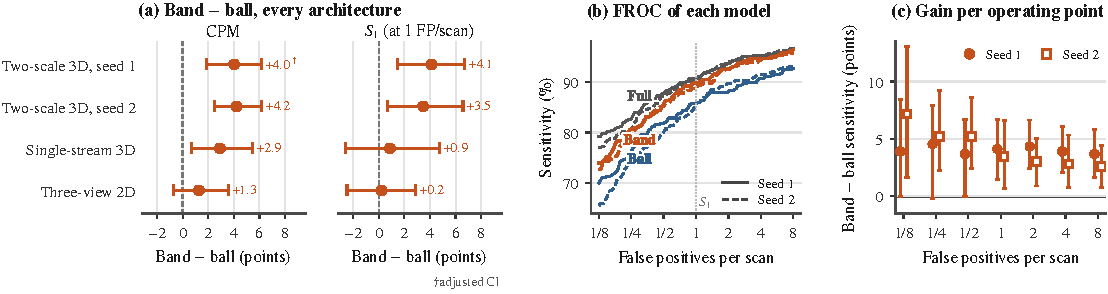
\includegraphics[width=\textwidth]{figures/restoration.pdf}
  \caption{Restoring the band improves two separately fitted two-scale 3D rankers on the same \EvalScans{} scans. A shows paired effects on CPM and sensitivity at matched 1 FP/scan. The primary CPM bar is adjusted across three locked comparisons. Other bars give pointwise 95\% patient intervals. B shows matched FROC for ball, ball plus band and full access, using both seeds. The band recovers \PrimaryRecovery\% and \RepeatRecovery\% of the observed full-minus-ball CPM gaps.}
  \label{fig:restoration}
\end{figure*}
\begin{table*}[t]
\centering
\small
\caption{Visibility on 353 reused scans. Absolute CPM is in percent. Paired band-minus-ball effects are in points. $^\dagger$ denotes the primary CPM interval adjusted across three locked contrasts. Other intervals are pointwise 95\%. Recovery is the band gain divided by the observed full-minus-ball CPM gap for each fit.}
\label{tab:visibility}
\begin{tabular}{@{}lrrrrrr@{}}
\toprule
Fitted architecture & Ball & Ball + band & Full & $\Delta$ CPM & $\Delta S_1$ & Recovery \\
\midrule
Two-scale 3D (3691) & 83.58 & 87.60 & 89.37 & $+4.03\,[1.85,\,6.17]$$^\dagger$ & $+4.12\,[1.45,\,6.71]$ & 70\% \\
Two-scale 3D (9143) & 82.83 & 87.05 & 88.63 & $+4.21\,[2.51,\,6.17]$ & $+3.47\,[0.67,\,6.59]$ & 73\% \\
Single-stream 3D (3691) & 80.94 & 83.85 & 85.84 & $+2.91\,[0.69,\,5.48]$ & $+0.87\,[-2.59,\,4.73]$ & 59\% \\
Three-view 2D (9143) & 81.28 & 82.55 & 84.75 & $+1.27\,[-0.71,\,3.58]$ & $+0.22\,[-2.49,\,2.88]$ & 37\% \\
\bottomrule
\end{tabular}
\end{table*}


The primary two-scale ranker achieves \BallCpm\% CPM with the native ball, \BandCpm\% with the ball and band, and \FullCpm\% with the full field (Fig.~\ref{fig:restoration} and Tab.~\ref{tab:visibility}). Restoring the band raises CPM by \RestorePrimary{} points under the three-contrast adjustment. The pointwise interval is \RestorePrimaryPointwise{} points. The second seed yields \RestoreRepeat{} points, using a pointwise interval. Matched $S_1$ gains are \RestoreOne{} and \RepeatOne{} points. All effects are calculated before rounding the absolute scores.

The absolute ranking curves separate across operating points, with higher sensitivity under restored access at all seven release rates in both fits. The gain represents \PrimaryRecovery\% and \RepeatRecovery\% of the observed gap from ball to full CPM. It leaves a residual advantage for the full crop. The recovery fraction refers to fitted ranking performance at the same proposals. It depends on the architecture, the training procedure and the operating points used in CPM. The band gains remain positive in each reused subset group and essentially unchanged when all marks are eligible. Supplement Sec.~S3 reports all seven operating points and the uncapped comparisons.

The independent-cutoff analysis separates a change in ranking from threshold calibration. Transferring each model's threshold selected on the 88 calibration scans changes sensitivity by \TransferredPrimary{} points for the primary fit and \TransferredRepeat{} points for the second. The achieved FP burdens differ by model. The two matched results therefore give stronger evidence for ranking improvement at 1 FP/scan than the fixed-threshold results give for deployment at a particular burden.

\subsection{Native source coverage matters at the same image entry point}
\label{sec:source_result}

\begin{figure*}[t]
  \centering
  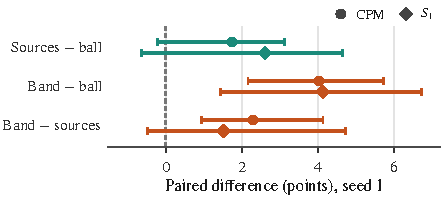
\includegraphics[width=\textwidth]{figures/coverage.pdf}
  \caption{Native query sources and the dense band enter the same image encoder. A counts distinct retained exterior native voxels per proposal that can contribute to the centered crop, averaged over the full evaluation stream. B gives paired CPM effects for the same two-scale 3D architecture and seed. All bars in B are pointwise 95\% patient intervals. The dense band outperforms exact query-source access even when both enter at the first image layer.}
  \label{fig:coverage}
\end{figure*}

A late residual could underperform simply because it receives sparse information after the image features have been computed. The native-source arm removes that difference in processing between the two image inputs. It retains the ball and the union of positive-weight sources of the same 384 query locations. Both this arm and the dense-band arm can learn spatial filters over all visible intensities from their first convolution. The mean exterior coverage reaching the centered crop is \QuerySources{} native sources per proposal in the query-source arm and \BandSources{} in the dense-band arm (Fig.~\ref{fig:coverage}).

Giving the encoder the query sources changes CPM over the ball by \SourcesGain{} points in the primary seed. The band adds a further \CoverageGap{} points over those sources. The point estimate for the latter comparison is positive in both subset groups, and removing the cap gives the same pooled CPM effect. At matched 1 FP/scan, query-source versus ball is \SourcesOne{} points and band versus query-source is \CoverageOne{} points. The CPM evidence is clearer than the result at that individual operating point.

The residual gap remains when the point of entry and image capacity are matched. It supports a role for the additional coverage and spatial continuity supplied by the dense band under this masking scheme. The holes between the retained query sources can disrupt patterns that a filter would otherwise see across the band. Their effect and that of the additional native measurements are coupled in this intervention. The query-source arm also retains the underlying HU values before sparse interpolation. Its comparison with the late endpoint heads combines changes in representation, fusion and the values available to the ranker.

\subsection{Relative geometry alone leaves a large sparse gap}
\label{sec:spatial_result}

\begin{figure*}[t]
  \centering
  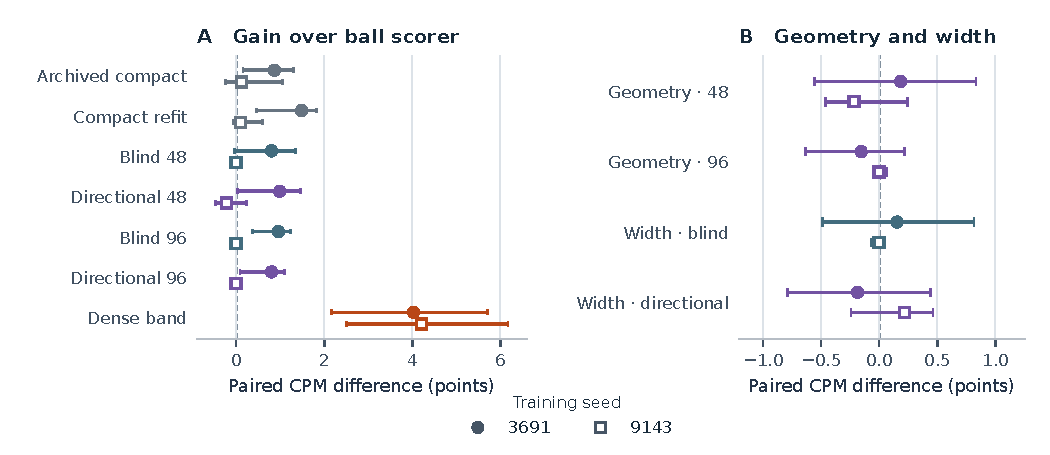
\includegraphics[width=\textwidth]{figures/spatial.pdf}
  \caption{Paired CPM effects of the same 384 readings on the two frozen ball scorers. A compares the archived compact head, its frozen-image refit and both widths of set attention against the same ball-only baseline. Dense restoration is shown on the same scale. B isolates the directional bias at fixed width and the width change at fixed bias. Pointwise 95\% intervals use shared patient draws. The two markers denote separate training seeds.}
  \label{fig:spatial}
\end{figure*}

Sparsity alone does not require pooling away angular structure. We test its value by adding relative directions to an otherwise identical attention head. The model can use line neighborhoods without relying on absolute orientation or learning a positional code from the ordering of the array. At width 48 the directional-minus-blind CPM effects are \GeometrySmallPrimary{} and \GeometrySmallRepeat{} points across the two seeds. At width 96 they are \GeometryLargePrimary{} and \GeometryLargeRepeat{} points. The matched $S_1$ differences also provide little evidence of a gain (supplement Sec.~S4). Doubling the width yields no consistent improvement in either geometry condition (Fig.~\ref{fig:spatial}B).

The compact refit changes CPM relative to the archived compact fit by \RefitPrimary{} and \RefitRepeat{} points. All refits share frozen image logits and the same sampling procedure. The primary compact refit gives the largest observed sparse gain over its ball scorer among the tested readouts for that seed. The dense band still leads the compact refits by \CompactGapPrimary{} and \CompactGapRepeat{} CPM points. The directional width-48 head trails the dense band by \ResidualSmallPrimary{} and \ResidualSmallRepeat{} CPM points and by \ResidualSmallOnePrimary{} and \ResidualSmallOneRepeat{} matched sensitivity points at 1 FP/scan. The width-96 comparison gives CPM gaps of \ResidualLargePrimary{} and \ResidualLargeRepeat{} points. These differences refer to the fitted readouts and use their unchanged ball-only references.

Taken together with the same-encoder source comparison, the attention experiments narrow the explanation. Giving a late readout the relative directions of the sampled axes, increasing its width and fitting after the image encoder converges leave a substantial CPM difference from dense access. The same backbone also benefits from denser access when all exterior evidence arrives before the first convolution. A more informative sampling pattern or a different geometry-preserving fusion could still use the existing budget of readings differently.

\subsection{The largest gains occur where the band reaches a lesion}
\label{sec:anatomy_result}

\begin{figure*}[t]
  \centering
  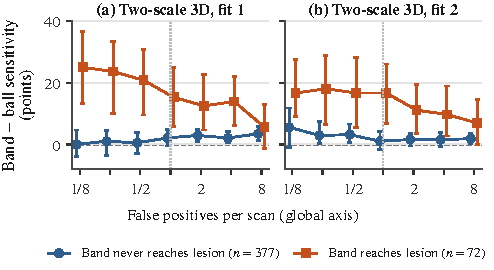
\includegraphics[width=\textwidth]{figures/anatomy.pdf}
  \caption{Anatomy groups defined from all original matching proposals before scores were joined. Sensitivity differences compare band and ball at global FP/scan targets on the complete streams. A lesion is in the overlap group if the band of any matching proposal reaches its majority-reader contour. The 377 never-overlap and 72 overlap lesions are shown, with paired pointwise 95\% patient intervals. The full FROC still includes the six unlinked lesions and the six linked lesions without proposals.}
  \label{fig:anatomy}
\end{figure*}
\begin{table*}[t]
\centering
\small
\caption{Lesion sensitivity at global 1 FP/scan, with a separate FROC curve for each model. All 461 lesions and all evaluated false marks contribute to the global curves. Effects are paired, with pointwise 95\% intervals.}
\label{tab:anatomy_one}
\begin{tabular}{@{}llrrrr@{}}
\toprule
Seed & Group & $n$ & Ball & Band & $\Delta S_1$ \\
\midrule
3691 & Never overlaps & 377 & 89.92 & 92.04 & $+2.12\,[-0.52,\,4.79]$ \\
3691 & Any overlap & 72 & 69.44 & 84.72 & $+15.28\,[5.81,\,25.00]$ \\
3691 & Linked, no proposal & 6 & 0.00 & 0.00 & $+0.00\,[0.00,\,0.00]$ \\
3691 & Unlinked & 6 & 100.00 & 100.00 & $+0.00\,[0.00,\,0.00]$ \\
9143 & Never overlaps & 377 & 89.92 & 90.98 & $+1.06\,[-1.68,\,4.27]$ \\
9143 & Any overlap & 72 & 69.44 & 86.11 & $+16.67\,[6.85,\,26.09]$ \\
9143 & Linked, no proposal & 6 & 0.00 & 0.00 & $+0.00\,[0.00,\,0.00]$ \\
9143 & Unlinked & 6 & 100.00 & 100.00 & $+0.00\,[0.00,\,0.00]$ \\
\bottomrule
\end{tabular}
\end{table*}


Of \EvalLesions{} reference lesions, 455 link to usable reader contours and 449 of those also have at least one matching proposal. The centered inference crop's visible band reaches majority-labeled lesion tissue at one or more matching proposals for \AnyOverlap{} of those 449. The other \NeverOverlap{} have no band overlap at any matching proposal. Across the entire pool there are 604 reference--proposal pairs, of which 598 have usable contours and 216 overlap. All six unlinked lesions have a matching proposal. The other six are linked lesions outside the proposal ceiling and remain in the denominator.

At 1 FP/scan, the band improves sensitivity in the overlap group by \AnyPrimary{} and \AnyRepeat{} points. The corresponding effects in the never-overlap group are \NeverPrimary{} and \NeverRepeat{} points. The overlap-minus-never difference in gains is \HeteroPrimary{} points in the primary fit and \HeteroRepeat{} in the second. Thus about one sixth of the reference lesions account for over half of the net increase at this target in each fit. The 8-FP pointwise estimates in the never-overlap group are positive with intervals above zero for both fits, while the estimates at 1 FP/scan are compatible with both small gains and small losses. Figure~\ref{fig:anatomy} shows the full range of operating points.

The median reference diameter is $17.36\mm$ in the overlap group and $5.75\mm$ in the never-overlap group. The overlap group also has more matching proposals per lesion. These properties can influence which lesions survive ranking under different visibility. The anatomy groups are observational, with imperfect contour coverage, and every sensitivity estimate also depends on the model's ranking of false marks. This supports the narrower explanation that the largest gains occur where restored voxels include part of the annotated lesion. It leaves the contribution of extra-lesional patterns to the gains unresolved. In the earlier descriptive decision audit at the primary discrete cutoff, the fitted band adds 28 lesions and loses nine. Of the 28 gained lesions, 12 have a highest-scoring retained mark whose band reaches the contour. The all-proposal grouping above is independent of that choice of mark.

\subsection{Transfer across image architectures}
\label{sec:breadth_result}

The distinct single-stream 3D architecture meets the prespecified 80\% full-visibility development criterion, with \SingleCheck\% and \SingleDev\% CPM on the checkpoint and readout development roles. On the evaluation pool, its band gains \SingleGain{} CPM points and \SingleOne{} points at matched 1 FP/scan (Tab.~\ref{tab:visibility}). Its CPM gain remains positive in both reused subset groups. A 3D model that processes the full field in a single hierarchy therefore also benefits from the intervention on the same proposal stream.

The earlier three-view fit gains \TriGain{} CPM points and \TriOne{} points at matched 1 FP/scan. This comparison is inconclusive. Each view uses a limited stack of central slices, so the same native mask is represented differently within the network. The architecture comparisons cover differences in how the resampled crop is processed while keeping patients and candidate locations fixed. The external eligibility recheck identified no untouched full-scan cohort with a usable reference and defensible evaluation route in the available inventories (supplement Sec.~S1).

\subsection{Compact controls and the full-context increment}
\label{sec:compact_result}

The original sparse factorial gives an adjusted endpoint-versus-scalar effect of \RepresentPrimary{} CPM points at fixed logit fusion. The second seed gives \RepresentRepeat{} points. The adjusted effect of embedding versus logit on the endpoint gain is \FusionPrimary{} points in the primary fit. These intervals and the change of sign across seeds leave the representation and conditioning advantages uncertain under this compact head. Paired-minus-sham CPM changes are \PairShamPrimary{} and \PairShamRepeat{} points, and the unpaired comparison is similarly uncertain. This leaves little evidence for a consistent advantage from the nominated opposing correspondence. Supplement Sec.~S3 gives the complete factorial and separately fitted controls.

Adding the paired head to full context with the selected gray-mean morphology term changes CPM by \PracticalPrimary{} and \PracticalRepeat{} points. Both upper interval endpoints fall below the prespecified $+1$ CPM-point target for the tested addition. That is a more precise statement than the representation and conditioning comparisons allow. Matched $S_1$ changes are \PracticalOne{} and \PracticalRepeatOne{} points. The low-FP noninferiority check clears its prespecified margin for the first fit, with a possible loss beyond the margin at the lowest rate for the second. Supplement Sec.~S3 reports the threshold transfer, sham and morphology comparisons.

\section{Discussion}
\label{sec:discussion}

\paragraph{What the band contributes.}
Limiting a ranker to a $10\mm$ native ball removes evidence that a wider view can recover. Restoring one thin band recovers about seven tenths of the CPM difference to the full field in two training runs, and the effect carries over to a single-stream 3D network. Sparse access, however it is read, recovers much less. Showing the image network the exact voxels behind the 384 samples closes less than half of the gap, and attention over sample directions adds little to a late readout. Reading a few well-chosen places, even with their geometry, is therefore not a substitute for seeing a contiguous region. A useful follow-up would vary the arrangement of visible voxels at a fixed count, separating coverage from continuity.

\paragraph{What ``exterior'' means for detection.}
The band lies outside a ball centred on the \emph{proposal}, not on the lesion. Large lesions and off-centre proposals put lesion tissue inside it, and this is where the largest gains occur, using a grouping fixed before scoring. Small benefits beyond the annotated lesion remain compatible with the data, especially at higher FP rates. The FROC changes could also come from better rejection of false proposals, even if a true proposal's own appearance were unchanged. Attributing gains to vessels, attachments or lesion margins would require other interventions or anatomical labels. For detector design, the result suggests checking how often proposals are displaced from the lesion centre before investing in long-range context modules.

\paragraph{Lesion size, proposal displacement and context.}
A $10\mm$ ball is wide enough to contain most small nodules, so for lesions below $6\mm$ the band adds only surroundings; all of them are in the never-reached group, whose gain at 1~FP/scan is small. For lesions of at least $10\mm$, the ball cuts through the nodule, and two thirds of them have lesion tissue in the band. Large lesions also attract more proposals: the 72 reached lesions have 221 matching proposals, whereas each never-reached lesion has exactly one. Many of these proposals lie away from the lesion centre, which is where the band restores lesion tissue. The context advantage reported for larger patches may therefore partly be a \emph{coverage} advantage for large lesions. Analyses of context in detection should report effects by lesion size, and patch sizes may be better chosen from the size distribution of the target lesions than from the scale of surrounding anatomy.

\paragraph{Limitations.}
Masking creates artificial air boundaries, and each model can adapt to them; the native-source and band conditions differ both in the voxels they show and in how these boundaries look after resampling. We tested one band, chosen to enclose the samples' support; other radii and equal-volume regions remain open. The sparse heads use unoriented axis pairs at one fusion point, so their results are specific to this design. In fit~2, three attention heads did not move from their initialization, which weakens the geometry evidence to fit~1 and the width-48 contrast. The native-source and single-stream comparisons each use one training seed, and the patient intervals do not capture variation across training runs. All fits share one candidate generator and one benchmark that has been studied before; an independent test would need an untouched full-scan cohort with a fixed proposal stream.

\section{Conclusion}
\label{sec:conclusion}

We asked what a wider view adds when a lung-nodule ranker scores fixed candidates, and answered it by changing only which native CT voxels the ranker can see. Restoring a thin, physically defined band around a $10\mm$ ball raises two-scale 3D CPM by about four points in two training runs and closes about 70\% of the gap to the full field; a second 3D architecture also gains. The dense band beats the exact voxels behind sparse samples in the same encoder, and adding sample geometry to sparse readouts does not close this gap. The largest gains occur where the band reaches annotated lesion tissue. Visibility interventions of this kind give a simple, architecture-independent way to ask which evidence a medical detector actually needs.


\section*{LLM Usage Statement}
\input{LLM_Usage_Statement.txt}

\clearpage
{\small
\bibliographystyle{ieeenat_fullname}
\bibliography{references}
}
\end{document}
